\documentclass[9pt]{beamer}
\usepackage[english, russian]{babel}
\usepackage[T2A]{fontenc}
\usepackage[utf8]{inputenc}
\usepackage{indentfirst}
\usepackage{amsmath, amsfonts, amssymb, amsthm, mathtools}
\usepackage[export]{adjustbox}
\usepackage{graphicx} 
\graphicspath{ {./images/} }

\usepackage{subcaption}
\usepackage{verbatim}

\usepackage{hyperref}

\hypersetup{
    colorlinks=true,
    linkcolor=blue,
    filecolor=magenta,      
    urlcolor=black,
    pdftitle={Overleaf Example},
    pdfpagemode=FullScreen,
    }

\usepackage[table]{xcolor}
\usepackage{array}
\usepackage{multirow}

\title{Лабораторная работа № 2. \\ Расчёт сети Fast Ethernet}
\author{Данила Стариков \\ НПИбд-02-22}
\date{2024}

\begin{document}

\maketitle
\newpage

\tableofcontents

\newpage
\section{Цель работы}
Цель данной работы — изучение принципов технологий Ethernet и Fast Ethernet
и практическое освоение методик оценки работоспособности сети, построенной
на базе технологии Fast Ethernet.

\newpage
\section{Выполнение работы}
\subsection{Постановка задачи}
Требуется оценить работоспособность 100-мегабитной сети Fast Ethernet в соответствии
с первой и второй моделями. Конфигурации сети приведены в табл. \ref{tab:netconfig}:
все сегменты соединены витой парой категории 5, длина приведена в метрах.
Топология сети представлена на рис. \ref{img:nettopology}.

\begin{table}[!ht]
    \caption{Варианты заданий}
    \label{tab:netconfig}
    \centering
    \begin{tabular}{|c|c|c|c|c|c|c|}
    \hline
        Вариант & Сегмент 1 & Сегмент 2 & Сегмент 3 & Сегмент 4 & Сегмент 5 & Сегмент 6 \\ \hline
        1 & 96 & 92 & 80 & 5 & 97 & 97 \\ \hline
        2 & 95 & 85 & 85 & 90 & 90 & 98 \\ \hline
        3 & 60 & 95 & 10 & 5 & 90 & 100 \\ \hline
        4 & 70 & 65 & 10 & 4 & 90 & 80 \\ \hline
        5 & 60 & 95 & 10 & 15 & 90 & 100 \\ \hline
        6 & 70 & 98 & 10 & 9 & 70 & 100 \\ \hline
    \end{tabular}
\end{table}

\begin{center}
    \centering
        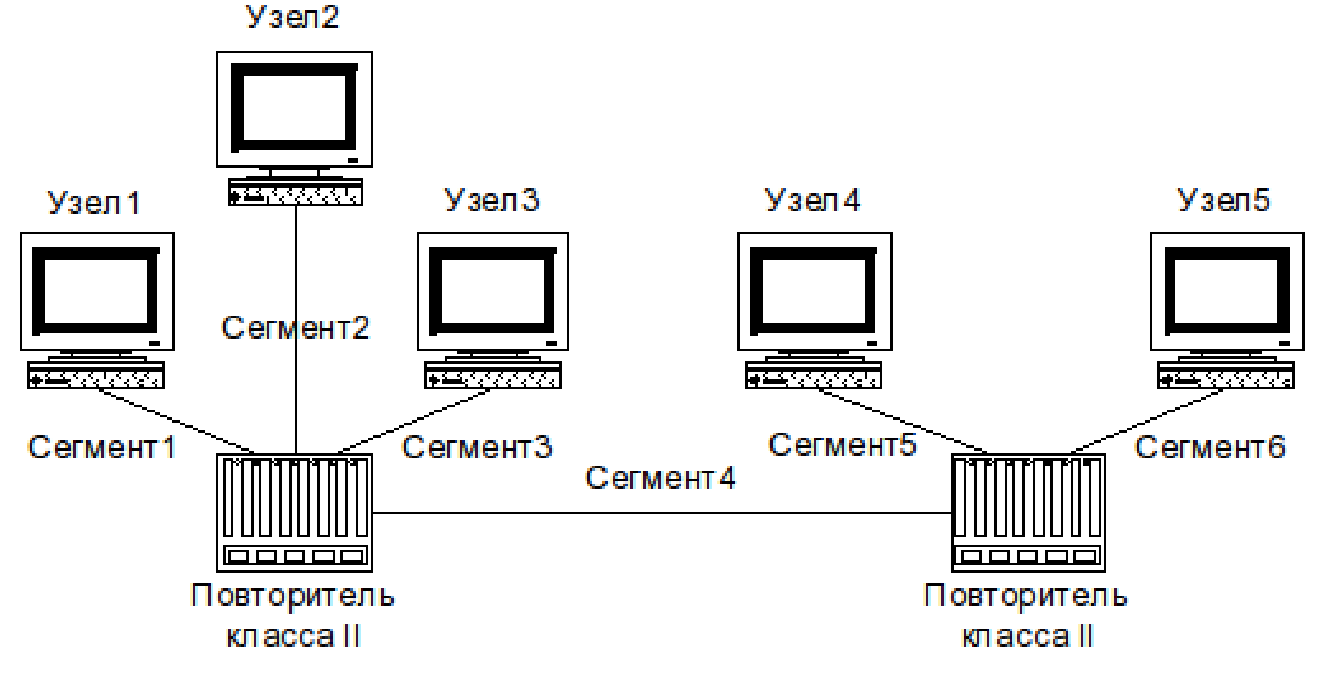
\includegraphics[width=\textwidth]{../images/topology.png}
    \captionof{figure}{Топология сети.}
    \label{img:nettopology}
\end{center}

\subsection{Проверка в соответствии с первой моделью сети Fast Ethernet}
Сеть считается работоспособной в соответствии с первой моделью при удовлетворении
следующих правил:
\begin{itemize}
    \item длина каждого сегмента витой пары должна быть меньше 100 м;
    \item длина каждого оптоволоконного сегмента должна быть меньше 412 м;
    \item если используются кабели MII (Media Independent Interface), то каждый из
        них должен быть меньше 0,5 м;

    \item задержки, вносимые кабелем MII, не учитываются при оценке временных
        параметров сети, так как они являются составной частью задержек, вносимых
        оконечными устройствами (терминалами) и повторителями.
\end{itemize}
    Стандартом определены два класса повторителей:
\begin{itemize}
    \item повторители класса I выполняют преобразование входных сигналов в цифровой
        вид, а при передаче снова перекодируют цифровые данные в физические
        сигналы; преобразование сигналов в повторителе требует некоторого времени,
        поэтому в домене коллизий допускается только один повторитель класса I;

    \item повторители класса II немедленно передают полученные сигналы без всякого
        преобразования, поэтому к ним можно подключать только сегменты, использующие
        одинаковые способы кодирования данных; можно использовать не
        более двух повторителей класса II в одном домене коллизий.
\end{itemize}

Также для нашей сети, которая содержит два повторителя класса II, предельно
допустимый диаметр домена коллизий должен быть меньше 205 м. Именно это и будет
основным критерием при проверке работоспособности сети.

Таблица \ref{tab:model1} содержит результаты проверки всех вариантов конфигурации
сети в соотвествии с первой моделью. Оранжевым цветом выделены сегменты, формирующие
домен коллизий, в последнем столбце красный цвет определяет варианты, которые
в соответствии с первой моделью не являются работоспособными, а именно №2, 5, 6.

\begin{table}[!ht]
    \caption{Проверка сети (Первая модель).}
    \label{tab:model1}
    \centering
    \begin{tabular}{|c|c|c|c|c|c|c|m{2cm}|}
    \hline
    Вар. & Сегмент 1 & Сегмент 2 & Сегмент 3 & \cellcolor{lightgray} Сегмент 4 & Сегмент 5 & Сегмент 6 & Диаметр домена коллизий \\ \hline
        1 &\cellcolor{orange} 96 & 92 & 80 &\cellcolor{orange} 5 &\cellcolor{orange} 97 & 97 & 198 \\ \hline
        2 &\cellcolor{orange} 95 & 85 & 85 &\cellcolor{orange} 90 & 90 &\cellcolor{orange} 98 & \cellcolor{red} 283 \\ \hline
        3 & 60 &\cellcolor{orange} 95 & 10 &\cellcolor{orange} 5 & 90 &\cellcolor{orange} 100 & 200 \\ \hline
        4 &\cellcolor{orange} 70 & 65 & 10 &\cellcolor{orange} 4 &\cellcolor{orange} 90 & 80 & 164 \\ \hline
        5 & 60 &\cellcolor{orange} 95 & 10 &\cellcolor{orange} 15 & 90 &\cellcolor{orange} 100 &\cellcolor{red} 209 \\ \hline
        6 & 70 &\cellcolor{orange} 98 & 10 &\cellcolor{orange} 9 & 70 &\cellcolor{orange} 100 &\cellcolor{red} 207 \\ \hline
    \end{tabular}
\end{table}

\subsection{Проверка в соответствии со второй моделью сети Fast Ethernet}
Проверка сети на работоспособность соответствии со второй моделью подразумевает
расчет времени двойного оборота сети при полудуплексном режиме обмена данными.
Время двойного оборота рассчитывается для наихудшего (в смысле распространения сигнала)
пути между двумя узлами домена коллизий. Расчёт выполняется путём суммирования
временных задержек в сегментах, повторителях и терминалах.
Сеть считается работоспособной, если время двойного оборота не превышает 512 би
(битовых интервала). Также рекомендуется добавить еще 4 би для учета непредвиденных
задежек. Таблица \ref{tab:data} содержит временные задержки компонентов, которые
потребуются для проверки сети.

\begin{table}[!ht]
    \caption{временные задержки компонентов сети}
    \label{tab:data}
    \centering
    \begin{tabular}{|l|l|}
    \hline
        Компонент пути & Время двойного оборота, би \\ \hline
        Пара терминалов с интерфейсами TX & 100 \\ \hline
        Сегмент на витой паре категории 5 ( на 1 метр) & 1.112 \\ \hline
        Повторитель класса II  & 92 \\ \hline
    \end{tabular}
\end{table}

Таблица \ref{tab:model2} содержит результат расчета времени двойного оборота для
всех вариантов конфигурации сети. Красным цветом отмечены варианты, время которых
превышает 512 би. Проверка в соответствии со второй моделью снова определила варианты
№ 2, 5, 6  как неработоспособные.
\begin{table}[!ht]
    \caption{Проверка сети (Вторая модель).}
    \label{tab:model2}
    \centering
    \begin{tabular}{|l|l|l|l|l|l|l|}
    \hline
    \multirow{3}{*}{Компонент пути} & \multicolumn{6}{|c|}{Время двойного оборота, би} \\ \cline{2-7}
                                    & \multicolumn{6}{|c|}{Вариант} \\ \cline{2-7}
                                    & 1 & 2 & 3 & 4 & 5 & 6 \\ \hline
        Пара терминалов с интерфейсами TX & 100 & 100 & 100 & 100 & 100 & 100 \\ \hline
        Первый сегмент на витой паре & 106.752 & 105.64 & 105.64 & 77.84 & 105.64 & 108.976 \\ \hline
        Второй сегмент на витой паре & 5.56 & 100.08 & 5.56 & 4.448 & 16.68 & 10.008 \\ \hline
        Третий сегмент на витой паре & 107.864 & 108.976 & 111.2 & 100.08 & 111.2 & 111.2 \\ \hline
        Повторитель класса II & 92 & 92 & 92 & 92 & 92 & 92 \\ \hline
        Повторитель класса II & 92 & 92 & 92 & 92 & 92 & 92 \\ \hline
        Врема двойного оборота сети, би & 504.176 & \cellcolor{red} 598.696 & 506.4 & 466.368 &\cellcolor{red} 517.52 &\cellcolor{red} 514.184 \\ \hline
    \end{tabular}
\end{table}


\newpage
\section{Выводы}
В рамках лабораторной работы изучили принципы технологии Ethernet и Fast Ethernet
и на практике познакомились с методиками оценки работоспособности сети, построенной
на базе технологии Fast Ethernet.
\end{document}
